% !TeX root = ./Report-Body.tex
\renewcommand{\arraystretch}{0.6}
\setlength\arraycolsep{2pt}
\renewcommand{\thefootnote}{\fnsymbol{footnote}}
\chapter{Derivation of Theory}
In order to gain a detailed, quantitative understanding of relaxation, it is necessary to delve into quantum mechanics. In this chapter, Bloch-Wangness-Redfield (BWR) Theory is introduced. A novel model specifically devised to describe the relaxation of a methyl or trifluoromethyl group within a molecule is presented. By establishing this theory, which incorporates both dipolar and CSA influences, it will become possible to establish which magnetisations are desirable to target during a $^{13}$CF$_3$ TROSY experiment.
\section{Spin Ensembles and the Density Matrix}
A nuclear spin, just like any other quantum system, is described by a wavefunction, $\ket{\Psi}$, which provides all discernible information about it. Any spin within an NMR sample will possess a wavefunction that consists of a linear combination of its basis eigenkets. For a spin-$\frac{1}{2}$ nucleus, this wavefunction takes a particularly simple form if we expand it in terms of the eigenkets of the $\hat{I}_z$ angular momentum operator:
\begin{equation}
\ket{\Psi}=c_{\alpha}\ket{\alpha}+c_{\beta}\ket{\beta}
\end{equation}
To describe NMR experiments, in which the system being studied comprises a very large ensemble of spins, in a mixed state, it is common practice to consider the \textit{density operator}, defined by:
\begin{equation}
\hat{\rho}=\overline{\ket{\Psi}\bra{\Psi}}
\end{equation}
where the overbar represents the average value for the entire ensemble\footnote{Note that in following sections, the overbar indicating ensemble averaging will sometimes be dropped for convenience, however this is implied throughout.}. The matrix representation of $\hat{\rho}$ features elements $\rho_{ba}=\overline{c_a^*c_b}$. For an ensemble of isolated spin-$\frac{1}{2}$ nuclei, $\hat{\rho}$ is given by:
\begin{equation}
\hat{\rho} = \mqty(\overline{\ket{\alpha}\bra{\alpha}} & \overline{\ket{\alpha}\bra{\beta}} \\ \overline{\ket{\beta}\bra{\alpha}} & \overline{\ket{\beta}\bra{\beta}}) = \mqty(\overline{c_{\alpha}^*c_{\alpha}} & \overline{c_{\beta}^*c_{\alpha}} \\ \overline{c_{\alpha}^*c_{\beta}} & \overline{c_{\beta}^*c_{\beta}})
\end{equation}
The ensemble-averaged expectation value of an observable corresponding to the operator $\hat{O}$, is given by:
\begin{equation}
\label{ExpVal}
\overline{\expval{\hat{O}}} = \text{Tr}\left[{\hat{\rho}\hat{O}}\right]
\end{equation}
The crux of NMR experiment analysis is to determine the time evolution of the density matrix during a pulse sequence. It then becomes possible to evaluate the expectation values of observables that are of interest, using \ref{ExpVal}.\\
It is common to represent the density operator as a linear combination of time-independent operators that form a complete basis, with time-dependent coefficients:
\begin{equation}
\hat{\rho} = \sum \limits_i c_i (t) \hat{O}_i
\end{equation}
where, for an ensemble of isolated spin-$\frac{1}{2}$ nuclei, the matrix representation of each operator, $\hat{O}_i$, is defined by:
\begin{equation}
\hat{O}_i = \mqty(\mel{\alpha}{\hat{O}_i}{\alpha} & \mel{\alpha}{\hat{O}_i}{\beta} \\ \mel{\beta}{\hat{O}_i}{\alpha} & \mel{\beta}{\hat{O}_i}{\beta})
\end{equation}
Two bases are conventionally used to describe an ensemble of spins, each one possessing four operators for an ensemble of isolated spin-$\frac{1}{2}$ nuclei. These are the Cartesian basis and the Single-element basis. Definitions of all the operators in these bases are defined as follows:\\
Cartesian basis:
\begin{equation}
\frac{1}{2}\hat{E} = \mqty(\frac{1}{2} & 0 \\ 0 & \frac{1}{2}) \hspace{20pt} \hat{I}_x = \mqty(0 & \frac{1}{2} \\ \frac{1}{2} & 0) \hspace{20pt} \hat{I}_y = i\mqty(0 & \frac{1}{2} \\ -\frac{1}{2} & 0) \hspace{20pt} \hat{I}_z = \mqty(\frac{1}{2} & 0 \\ 0 & -\frac{1}{2})
\end{equation}
Single-element basis:
\begin{equation}
\hat{I}^{\alpha} = \frac{1}{2} \hat{E} + \hat{I}_z \hspace{20pt} \hat{I}^{\beta} = \frac{1}{2} \hat{E} - \hat{I}_z \hspace{20pt} \hat{I}^+ = \hat{I}_x + i\hat{I}_y \hspace{20pt} \hat{I}^- = \hat{I}_x - i\hat{I}_y 
\end{equation}
The complete density matrix of an ensemble of isolated spin-$\frac{1}{2}$ nuclei is therefore given by:
\begin{equation}
\hat{\rho} = \frac{1}{2} c_E \hat{E} + c_x \hat{I}_x + c_y \hat{I}_y + c_z \hat{I}_z = c_{\alpha} \hat{I}^{\alpha} + c_{\beta} \hat{I}^{\beta} + c_+ \hat{I}^+ + c_- \hat{I}^-
\end{equation} 
\subsection{Multi-spin Systems}
To construct wave functions describing a system of multiple scalar-coupled spins, direct (Kronecker) products of the relevant single-spin wavefunctions are taken. For an N-spin system:
\begin{equation}
\ket{\Psi_{N\text{-spin}}} = \ket{\psi_1} \otimes \ket{\psi_2} \otimes ... \otimes \ket{\psi_N}
\end{equation}
In general, the density matrix describing an ensemble of $N$ scalar-coupled spin-$\frac{1}{2}$ nuclei is $2^N \times 2^N$ in dimension, and described by a linear combination of $4^N$ operators. These operators are formed by taking Kronecker products of the single spin operators descried above.
The spin systems of primary interest in this thesis ($^{13}$CH$_3$ and $^{13}$CF$_3$) consist of 4 spin-$\frac{1}{2}$ nuclei. As such, a complete density matrix describing these systems is $16 \times 16$ in dimension, and composed of a linear combination of $256$ product operators.
\section{Time Dependence of the Density Matrix}
The time-dependence of the density operator, under the influence of a Hamiltonian, $\hat{H}$, is described by the Liouville-von Neumann equation\cite{RN39}:
\begin{equation}
\dv{\hat{\rho}}{t}=-i\comm{\hat{H}}{\hat{\rho}}
\end{equation}
A common treatment of the Hamiltonian in the context of spin dynamics is to assume that it is composed of two separate parts:
\begin{equation}
\begin{split}
\hat{H} (t) &= \hat{H}_0 + \hat{H}_1 (t) \\
\therefore \dv{\hat{\rho} (t)}{t} &= -i \left\lbrace\comm{\hat{H}_0}{\hat{\rho (t)}} + \comm{\hat{H}_1 (t)}{\hat{\rho (t)}}\right\rbrace
\end{split}
\end{equation}
where $\hat{H}_0$ describes all the time-independent contributions to the Hamiltonian, and $\hat{H}_1 (t)$ describes the time-dependent contributions, arising from random fluctuations in local magnetic fields within the sample. It should be noted that the time-averaged value of $\hat{H}_1 (t)$, given by $\overline{\hat{H}_1(t)}$ is 0. As such, $\hat{H}_1 (t)$ has no bearing on the position or number of peaks in spectra, though it plays a key role in the relaxation of nuclear spin systems.
The most widely utilised theory for the study of nuclear spin relaxation was devised by Bloch, Wangsness and Redfield\cite{RN23,RN13}. The key result of BWR theory is the following expression describing the time-dependence of the density matrix: 
\begin{equation}
\label{superoperator}
\begin{gathered}
\pdv{\hat{\rho}(t)}{t} = -i \comm{\hat{H}_0}{\hat{\rho} (t)} - \hat{\hat{\Gamma}}(\hat{\rho} (t) - \hat{\rho}_{\text{eq}}) \\
\hat{\hat{\Gamma}} = \int \limits_0^{\infty} \overline{\comm{\hat{H}_1 (t)^{\dagger}}{\comm{e^{-i \hat{H}_0 \tau} \hat{H}_1 (t - \tau)  e^{i \hat{H}_0 \tau}}{}}} d \tau
\end{gathered}
\end{equation}
where $\hat{\hat{\Gamma}}$ is the \textit{relaxation superoperator},  and $\hat{\rho}_{\text{eq}}$ is the density matrix of the ensemble in its equilibrium state. A derivation of this result is outlined in Appendix A. The matrix form of $\hat{\hat{\Gamma}}$ comprises elements $\Gamma_{rs}$ defined by:
\begin{equation}
\Gamma_{rs} = \frac{\mel{\hat{\rho}_s}{\hat{\hat{\Gamma}}}{\hat{\rho}_r}}{\sqrt{\bra{\hat{\rho}_r} \ket{\hat{\rho}_r} \bra{\hat{\rho}_s} \ket{\hat{\rho}_s}}}
\end{equation}
\section{Hamiltonians in Relaxation}
It is necessary to derive the form of $\hat{H}_1(t)$, the operator which describes the stochastically fluctuating local interactions within an NMR sample. Hamiltonians that describe the relevant interactions which induce relaxation need to be established. Common examples of such interactions include the dipolar interaction, the chemical shift anisotropy, and the quadrupolar interaction. This thesis focusses solely on spin-$\frac{1}{2}$ nuclei. As such, the quadrupolar interaction, which only applies when considering nuclei that are spin-$1$ or higher, will not be considered. Following this, we must perform rotations on the Hamiltonian, in order to imitate the motion of the molecule in solution, to work out their effects on relaxation.
\subsection{Hamiltonians in Spin Dynamics}
It is necessary to consider the different contributions to the stochastic Hamiltonian, $\hat{H}_1 (t)$, in order to describe relaxation phenomena successfully. Fortunately, there is a general framework which can be applied to all Hamiltonians relevant to spin-relaxation. Any such Hamiltonian may be expressed as follows:
\begin{equation}
\hat{H}=\vec{I}^\intercal \cdot \hat{A} \cdot \vec{S}
\end{equation}
$\vec{I}$ and $\vec{S}$ are vectors which describe the two interacting entities. These would represent two distinct spins in the case for the dipolar interaction. When considering the CSA, they would represent a spin and the external magnetic field, respectively. $\hat{A}$ is a second rank tensor that characterises the interaction. In a Cartesian axis system, the explicit form of the Hamiltonian is defined by:
\begin{equation}
\hat{H} = \mqty(\hat{I}_x & \hat{I}_y & \hat{I}_z) \mqty(A_{xx} & A_{xy} & A_{xz} \\ A_{yx} & A_{yy} & A_{yz} \\ A_{zx} & A_{zy} & A_{zz}) \mqty(\hat{S}_x \\ \hat{S}_y \\ \hat{S}_z)
\end{equation}
The values of the elements within the tensor $\hat{A}$ are dependent on the co-ordinate system in which we cast it. The simplest co-ordinate system possible is such that the interaction tensor is diagonal, which is known as its \textit{Principal Axis Frame} (PAF):
\begin{equation}
\label{PAFtensor}
\hat{A}_{\text{PAF}} = \mqty(A_{11} & 0 & 0 \\ 0 & A_{22} & 0 \\ 0 & 0 & A_{33})
\end{equation}
It is possible to split \ref{PAFtensor}, by defining three properties of the tensor; the \textit{isotropy}, the \textit{anisotropy}, and the \textit{asymmetry}:
\begin{equation}
\label{IsoAnisoAsymm}
A_{\text{iso}} = \frac{1}{3} (A_{11} + A_{22} + A_{33}) \hspace{15pt} A_{\text{aniso}} = \frac{1}{3} (A_{33} - A_{11}) \hspace{15pt} A_{\text{asymm}} = \frac{A_{22} - A_{11}}{A_{33} - A_{11}}
\end{equation}
Using the quantities defined in \ref{IsoAnisoAsymm}, $\hat{A}_{\text{PAF}}$ can be written as:
\begin{equation}
\label{PAFtensor_broken}
\hat{A}_{\text{PAF}} = A_{\text{iso}} \mqty(\imat{3}) + A_{\text{aniso}} \mqty(-1 & 0 & 0 \\ 0 & -1 & 0 \\ 0 & 0 & 2) + A_{\text{asymm}} A_{\text{aniso}} \mqty(1 & 0 & 0 \\ 0 & -2 & 0 \\ 0 & 0 & 1)
\end{equation}  
Whilst the PAF is the most convenient way to express a particular Hamiltonian, it necessary to express the Hamiltonian in terms of a set of co-ordinates that rotate relative to the internal co-ordinates of the molecule. We call such a system the \textit{Laboratory Frame}. However, before converting to the laboratory frame, establishment of the fixed orientations of the interaction tensors relative to each other is required. Doing this brings the system into the \textit{Molecular Frame}. In the following section, the necessary theory of rotations required to achieve such transformations is outlined. 
\subsection{Relevant Theory of Rotations}
A general rotation, by Euler angles $(\alpha$, $\beta$, $\gamma)$, applied to a Hamiltonian is given by:
\begin{equation}
\hat{H}_{\text{rot}} = \hat{\hat{R}}(\alpha, \beta, \gamma)[\vec{I}^{\intercal}\cdot\hat{A}\cdot\vec{S}] = \vec{I}^{\intercal} \cdot \hat{R}(\alpha, \beta, \gamma) \hat{A} \hat{R}^{-1}(\alpha, \beta, \gamma) \cdot \vec{S}
\end{equation}
The $z$-$y$-$z$ convention is commonly used, where an object is first rotated by the angle $\gamma$ about the $z$-axis, then by the angle $\beta$ about the $y$-axis, and finally by the angle $\alpha$ about the $z$-axis. As such, $\hat{R}(\alpha, \beta, \gamma)$ is defined by:
\begin{equation}
\hat{R}(\alpha, \beta, \gamma) = \mqty(\cos \alpha & -\sin \alpha & 0 \\ \sin \alpha & \cos \alpha & 0 \\ 0 & 0 & 1) \mqty(\cos \beta & 0 & -\sin \beta \\ 0 & 1 & 0 \\ \sin \beta & 0 & \cos \beta) \mqty(\cos \gamma & -\sin \gamma & 0 \\ \sin \gamma & \cos \gamma & 0 \\ 0 & 0 & 1)
\end{equation}
Whilst performing rotations on the PAF Hamiltonian in the form already presented is perfectly valid, these rotations will be far more manageable by changing the basis of operators that are used to describe it. The basis of choice is that of the \textit{irreducible spherical tensor operators}. There are 5 2$^{\text{nd}}$-rank spherical tensor operators, $\hat{T}_k^{(2)}$, where $k$ takes the values $-2$ to $2$ in integer steps. 
The result of applying a general rotation by Euler angles $(\alpha$, $\beta$, $\gamma)$ on a spherical tensor operator of rank 2 is as follows:
\begin{equation}
\hat{\hat{R}}(\alpha, \beta, \gamma) \hat{T}_{k}^{(2)} = \sum \limits_{k{\prime} = -2}^2 \mathfrak{D}_{k{\prime},k}^{(2)}(\alpha, \beta, \gamma) \hat{T}_{k{\prime}}^{(2)}
\end{equation}
Where $\mathfrak{D}_{k{\prime},k}^{(2)}(\alpha, \beta, \gamma)$ are the elements of the the $\text{2}^{\text{nd}}$-rank Wigner D-Matrix. The elements of this matrix are related to those of the reduced $\text{2}^{\text{nd}}$-rank Wigner Matrix, $d_{k{\prime},k}^{(2)}(\beta)$, according to:
\begin{equation}
\mathfrak{D}_{k{\prime},k}^{(2)}(\alpha, \beta, \gamma) = e^{-i k{\prime} \alpha} d_{k{\prime},k}^{(2)}(\beta) e^{-i k \gamma}
\end{equation}
Where the reduced $\text{2}^{\text{nd}}$-rank Wigner Matrix is defined as follows:
\begin{equation}
\label{RedWignerMatrix}
\mqty(\frac{(1 + \cos\beta)^2}{4} & -\frac{(1+\cos\beta)\sin\beta}{2} & \sqrt{\frac{3}{8}}\sin^2\beta & -\frac{(1-\cos\beta)\sin\beta}{2} & \frac{(1-\cos\beta)^2}{4} \\ \frac{(1+\cos\beta)\sin\beta}{2} & \frac{cos\beta - 1}{2} + \cos^2\beta & -\sqrt{\frac{3}{8}}\sin2\beta & \frac{\cos\beta + 1}{2} - \cos^2\beta & -\frac{(1 - \cos\beta)\sin\beta}{2} \\ \sqrt{\frac{3}{8}}\sin^2\beta & \sqrt{\frac{3}{8}}\sin2\beta & \frac{3\cos^2\beta - 1}{2} & -\sqrt{\frac{3}{8}}\sin2\beta & \sqrt{\frac{3}{8}}\sin^2\beta \\ \frac{(1 - \cos\beta)\sin\beta}{2} & \frac{\cos\beta + 1}{2} - \cos^2\beta & \sqrt{\frac{3}{8}}\sin2\beta & \frac{\cos\beta - 1}{2} + \cos^2\beta & -\frac{(1 + \cos\beta)\sin\beta}{2} \\ \frac{(1 - \cos\beta)^2}{4} & \frac{(1 - \cos\beta)\sin\beta}{2} & \sqrt{\frac{3}{8}}\sin^2\beta & \frac{(1 + \cos\beta)\sin\beta}{2} & \frac{(1 + \cos\beta)^2}{4})
\end{equation}
Some of the spherical tensor operators consist of sums of linear combinations of operators. It will become highly beneficial when deriving an expression for $\hat{\hat{\Gamma}}$ to split these particular tensors into terms containing single operators, as follows:
\begin{equation}
\hat{T}_k^{(2)} = \sum \limits_n \hat{T}_{k,n}^{(2)}
\end{equation}
The full set of $\hat{T}_{k,n}^{(2)}$ terms are given in Table \ref{SphericalOperators}.\\
\begin{table}[]
\centering
\begin{tabular}{l|lll}
       & $n = 1$ & $n = 2$ & $n = 3$ \\ \hline
$k=-2$ & $\frac{1}{2} \hat{I}^{-} \hat{S}^{-}$      & -       & -       \\
$k=-1$ & $\frac{1}{2} \hat{I}_z \hat{S}^{-}$      & $\frac{1}{2} \hat{I}^{-} \hat{S}_{z}$      & -       \\
$k=0$  & $\sqrt{\frac{2}{3}} \hat{I}_{z} \hat{S}_{z}$      & $-\frac{1}{4} \sqrt{\frac{2}{3}} \hat{I}^{+} \hat{S}^{-}$      & $-\frac{1}{4} \sqrt{\frac{2}{3}} \hat{I}^{-} \hat{S}^{+}$      \\
$k=1$  & $-\frac{1}{2} \hat{I}_z \hat{S}^{+}$      & $-\frac{1}{2} \hat{I}^{+} \hat{S}_z$      & -       \\
$k-2$  & $\frac{1}{2} \hat{I}^{+} \hat{S}^{+}$      & -       & -      
\end{tabular}
\caption{The full set of terms, $T_{k,n}^{(2)}$, that make up the spherical tensor operators, $\hat{T}_k^{(2)}$. The range of values $n$ takes depends on the value of $k$. For $k = \pm 2$, $n=1$ only. For $k = \pm 1$, $n=1, 2$. Finally, for $k = 0$, $n=1, 2, 3$.}
\label{SphericalOperators}
\end{table}
\subsection{Transforming a Hamiltonian into the Molecular Frame}
With this framework for rotations established, we now look to express $\hat{H}_{\text{PAF}}$ in terms of spherical tensor operators. Using the definition of $\hat{A}_{\text{PAF}}$ in \ref{PAFtensor_broken}, $\hat{H}_{\text{PAF}}$ takes the following form:
\begin{equation}
\begin{split}
\hat{H}_{\text{PAF}} = &\underbrace{A_{\text{iso}}\left(\hat{I}_x \hat{S}_x + \hat{I}_y \hat{S}_y + \hat{I}_z \hat{S}_z\right)}_{\tiny\textcircled{1}}  + \underbrace{A_{\text{aniso}}\left(-\hat{I}_x \hat{S}_x - \hat{I}_y \hat{S}_y + 2\hat{I}_z \hat{S}_z\right)}_{\tiny\textcircled{2}} \\ &+ \underbrace{A_{\text{aniso}} A_{\text{asymm}} \left(\hat{I}_x \hat{S}_x - 2\hat{I}_y \hat{S}_y + \hat{I}_z \hat{S}_z\right)}_{\tiny\textcircled{3}}
\end{split}
\end{equation}
By noting the relations $\hat{I}_x \hat{S}_x = \frac{1}{4}\left(\hat{I}^+ + \hat{I}^-\right)\left(\hat{S}^+ + \hat{S}^-\right)$ and \\$\hat{I}_y \hat{S}_y = -\frac{1}{4}\left(\hat{I}^+  - \hat{I}^-\right)\left(\hat{S}^+ - \hat{S}^-\right)$, the components of the Hamiltonian that are affected by rotation\footnote{The isotropic component of a Hamiltonian, \textcircled{1}, is invariant to rotation, and as such does not contribute to relaxation. It is incorporated in the time-independent Hamiltonian, $\hat{H}_0$.} can be re-expressed as follows:
\begin{equation}
\begin{split}
&\textcircled{2} =\sqrt{6}A_{\text{aniso}}\hat{T}_0^{(2)} \\
&\textcircled{3} = \frac{1}{2} A_{\text{aniso}} A_{\text{asymm}} \left(3 (\hat{T}_2^{(2)} + \hat{T}_{-2}^{(2)}) - \sqrt{6} \hat{T}_0^{(2)} \right)
\end{split}
\end{equation}
In this thesis it is assumed that all contributions to $\hat{H}_1 (t)$ solely have an anisotropic contribution\footnote{A useful simplification arises by assuming that the interaction tensors are axially symmetric (i.e. $A_{\text{asymm}} = 0$). A rotation of an axially symmetric tensor, aligned along the $z$-axis, about the $z$-axis has no effect. We therefore only require two angles to describe the rotation of such tensors, $\beta$ and $\alpha$. These correspond to the polar ($\theta$) and azimuthal ($\phi$) angles used in the spherical polar co-ordinate system.}, such that:
\begin{equation}
\hat{H}_{\text{PAF}} = \hat{H}_{\text{iso}} + \sqrt{6} A_{\text{aniso}}\hat{T}_0^{(2)}
\end{equation}
In order to bring the Hamiltonian into the molecular frame, a time-independent rotation, $\Omega$, is applied to it: 
\begin{equation}
\label{MolFrameHam}
\hat{H}_{\text{mol}} = \hat{H}_{\text{iso}} + \sqrt{6} A_{\text{aniso}} \sum \limits_{k = -2}^2 \mathfrak{D}_{k,0}^{(2)}(\Omega) \sum \limits_n \hat{T}_{k,n}^{(2)}
\end{equation}
where $\Omega = (\alpha, \beta)$ 
\subsection{Bringing a Hamiltonian into the Laboratory Frame}
A general interaction Hamiltonian in the Laboratory frame is generated by rotating \ref{MolFrameHam} in a way that mimics the motion of the system of interest. This is achieved by applying time-dependent rotations to the Hamiltonian. If a single 'type' of motion occurs, the Laboratory Frame Hamiltonian takes the form:
\begin{equation}
\label{LabFrameHamIso}
\hat{H}_{\text{Lab}} = \hat{H}_{\text{iso}} + \sqrt{6}A_{\text{aniso}} \sum \limits_{m = -2}^2 \sum \limits_{k = -2}^2  \mathfrak{D}_{m,k}^{(2)}(t) \mathfrak{D}_{k,0}^{(2)} (\Omega) \sum_n\hat{T}_{k,n}^{(2)}
\end{equation}
This form is appropriate for describing a Hamiltonian following the global rotation of the molecule, with the absence of any locally defined motion affecting it. For example, $^{15}$N-$^1$H pairs in the amide backbone can be adequately described in this fashion. In contrast, describing the motion of I$_3$S spin systems, such as methyl groups, is not appropriate using \ref{LabFrameHamIso}. In this case, the methyl group rotates rapidly about its threefold symmetry axis, whilst also following the global motion of the molecule as a whole. An extra rotation to account for this methyl rotation is necessary. To consider the form of such a Hamiltonian, we start, again, at \ref{MolFrameHam}. To describe the motion of the I$_3$S moiety, this Hamiltonian is operated on by a rotation, $\hat{\hat{R}}_{\text{methyl}}$: 
\begin{equation}
\hat{H}_{\text{Lab}} = \hat{H}_{\text{iso}} + \sqrt{6} A_{\text{aniso}} \hat{\hat{R}}_{\text{methyl}} \sum \limits_{k = -2}^2 \mathfrak{D}_{k,0}^{(2)}(\Omega) \sum \limits_n \hat{T}_{k,n}^{(2)}
\end{equation}
\begin{figure}
\centering
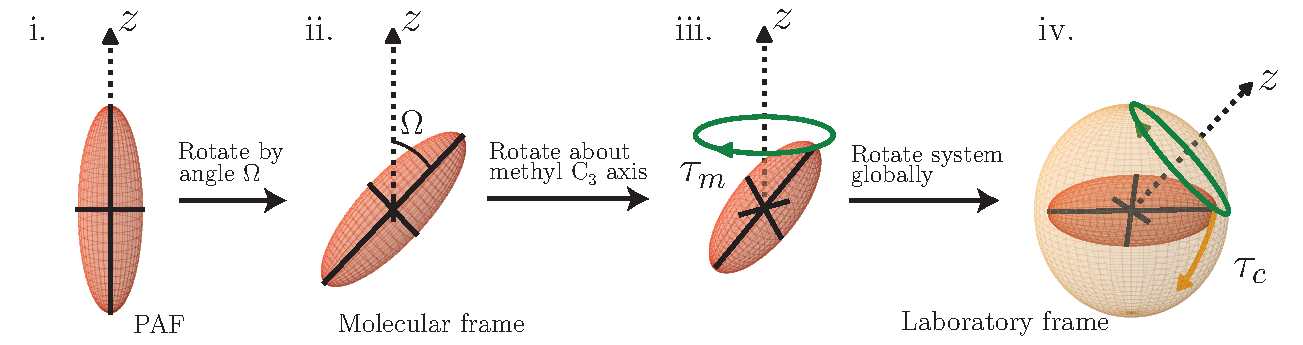
\includegraphics[scale=0.65]{./Figures/SimonsFigs/Rotations.pdf}
\caption{The sequence of rotations applied to the interaction tensors using the methyl rotation model. i. The tensor is initially aligned along the $z$-axis of the PAF. ii. It is then rotated into the molecular frame by the angle $\Omega(\alpha,\beta)$. iii. It is then allowed to rotate about the $z$-axis, which is defined to be the threefold rotation axis of the methyl group, characterised by correlation time $\tau_{\text{m}}$. iv. Finally, the whole system is allowed to undergo spherical isotropic motion, characterised by correlation time $\tau_{\text{c}}$.}
\label{Rotations}
\end{figure}
The $z$-axis is assumed to be the methyl rotation axis. As a result,  the angle $\beta$, which describes rotation about the $y$-axis, is set to $0$. Only diagonal elements of the Wigner D-Matrix which describe rotation about the methyl axis will be non-zero, which can be seen by inspecting \ref{RedWignerMatrix}. Incorporating methyl rotation, and subsequently global tumbling into the Hamiltonian therefore yields:
\begin{equation}
\hat{H}_{\text{Lab}} = \hat{H}_{\text{iso}} + \sqrt{6} A_{\text{aniso}} \hat{\hat{R}}_{\text{c}} \hat{\hat{R}}_{\text{m}} \sum \limits_{k = -2}^2 \mathfrak{D}_{k,0}^{(2)}(\Omega) \sum \limits_n \hat{T}_{k,n}^{(2)}
\end{equation}
where the rotation matrices, $\hat{\hat{R}}_{\text{m}}$  and $\hat{\hat{R}}_{\text{c}}$, which correspond to local methyl rotation and global tumbling respectively, are given by:
\scriptsize
\begin{equation}
\hat{\hat{R}}_{\text{m}} = \mqty(\mathfrak{D}_{-2,-2}^{(2) \text{m}} & 0 & 0 & 0 & 0 \\ 0 & \mathfrak{D}_{-1,-1}^{(2) \text{m}} & 0 & 0 & 0 \\ 0 & 0 & \mathfrak{D}_{0,0}^{(2) \text{m}} & 0 & 0 \\ 0 & 0 & 0 & \mathfrak{D}_{1,1}^{(2) \text{m}} & 0 \\ 0 & 0 & 0 & 0 & \mathfrak{D}_{2,2}^{(2) \text{m}}),
\hat{\hat{R}}_{\text{c}} = \mqty(\mathfrak{D}_{-2,-2}^{(2) \text{c}} & \mathfrak{D}_{-2,-1}^{(2) \text{c}} & \mathfrak{D}_{-2,0}^{(2) \text{c}} & \mathfrak{D}_{-2,1}^{(2) \text{c}} & \mathfrak{D}_{-2,2}^{(2) \text{c}} \\ \mathfrak{D}_{-1,-2}^{(2) \text{c}} & \mathfrak{D}_{-1,-1}^{(2) \text{c}} & \mathfrak{D}_{-1,0}^{(2) \text{c}} & \mathfrak{D}_{-1,1}^{(2) \text{c}} & \mathfrak{D}_{-1,2}^{(2) \text{c}} \\ \mathfrak{D}_{0,-2}^{(2) \text{c}} & \mathfrak{D}_{0,-1}^{(2) \text{c}} & \mathfrak{D}_{0,0}^{(2) \text{c}} & \mathfrak{D}_{0,1}^{(2) \text{c}} & \mathfrak{D}_{0,2}^{(2) \text{c}} \\ \mathfrak{D}_{1,-2}^{(2) \text{c}} & \mathfrak{D}_{1,-1}^{(2) \text{c}} & \mathfrak{D}_{1,0}^{(2) \text{c}} & \mathfrak{D}_{1,1}^{(2) \text{c}} & \mathfrak{D}_{1,2}^{(2) \text{c}} \\ \mathfrak{D}_{2,-2}^{(2) \text{c}} & \mathfrak{D}_{2,-1}^{(2) \text{c}} & \mathfrak{D}_{2,0}^{(2) \text{c}} & \mathfrak{D}_{2,1}^{(2) \text{c}} & \mathfrak{D}_{2,2}^{(2) \text{c}}) 
\end{equation}
\normalsize
An illustration describing the various rotation processes that are applied to an interaction tensor, using this model, is presented in Figure \ref{Rotations}. The Hamiltonian, for an individual interaction, using the methyl rotation model is therefore given by:
\begin{equation}
\label{MethylHam}
\hat{H}_{\text{Lab}} = \hat{H}_{\text{iso}} + \sqrt{6} A_{\text{aniso}} \sum \limits_{m = -2}^2 \sum \limits_{k = -2}^2 \mathfrak{D}_{m,k}^{(2) \text{c}}(t) \mathfrak{D}_{k,k}^{(2) \text{m}}(t) \mathfrak{D}_{k,0}^{(2)}(\Omega) \sum \limits_n \hat{T}_{k,n}^{(2)}
\end{equation}
\subsection{Relaxation-Inducing Interactions}
With the general framework established above, it is now a good time to consider some specific interactions that are of interest in the context of nuclear spin relaxation.
\subsubsection{The Dipolar Interaction}
\begin{figure}
\centering
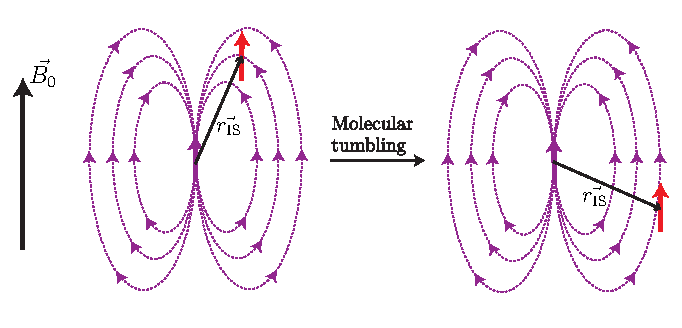
\includegraphics[scale=0.9]{./Figures/SimonsFigs/Dipolar.pdf}
\caption{An illustration of the dipolar interaction between two spins. Each dipole experiences the magnetic field emanating from the other dipole. The instantaneous magnetic field that the red spin experiences from the purple spin changes with time, due to molecular motion. It is this fluctuation in the local magnetic field that induces relaxation. Note that in this case, the two spins are assumed to be separated by a constant distance, as a result of chemical bonding.}
\label{Dipolar}
\end{figure}
The dipolar interaction is the direct interaction between two magnetic dipoles, as a result of one of the dipoles experiencing the magnetic field emanating from the other dipole, and vice-versa. The interaction is time-averaged to zero in solution, as the interaction is modulated by molecular diffusion. Despite this, the instantaneous dipolar interaction that two spins experience at any given time is one of the key mechanisms that induces relaxation in NMR. This principle is illustrated in Figure \ref{Dipolar}.\\
The anisotropy constant, $A_{\text{aniso}}^{\text{dipolar}} = d_{\text{IS}}$, is given by:
\begin{equation}
\label{DipConst}
d_{\text{IS}} = \left(\frac{\mu_0}{4 \pi}\right) \frac{\gamma_{\text{I}} \gamma_{\text{S}} \hbar}{r_{\text{IS}}^3}
\end{equation}
where $\gamma_{\text{I}}$ and $\gamma_{\text{S}}$ are the \textit{gyromagnetic ratios} of the two spins, and $r_{\text{IS}}$ is the distance that separates them. Note that the dipolar interaction does not feature an asymmetric component.
\subsubsection{The Chemical Shift Interaction}
The chemical shift interaction describes the generation of secondary magnetic fields about nuclear spins as a result of the motion of electrons induced by the external magnetic field, $\vec{B_0}$. This interaction, whilst also having an isotropic component, which directly impacts the position of peaks in spectra, often possesses both anisotropic and asymmetric components. This is a result of an uneven distribution electron density about a nucleus. However, it will be assumed that the chemical shift tensor is axially symmetrical, which is a treatment commonly adopted. The constant $A_{\text{aniso}}^{\text{CS}} = c_{\text{I}}$ is given by:
\begin{equation}
\label{CSAConst}
c_{\text{I}} = \gamma_{\text{I}} B_0 \Delta \sigma_{\text{I}}
\end{equation}
where $B_0$ is the magnetic field strength and $\Delta \sigma_{\text{I}}$, the anisotropy of the tensor, is given by $A_{33} - A_{11}$.
\section{Relaxation Models} \label{RelaxModels}
\subsection{Spherical Isotropic Motion} \label{SphericalSuperoperator}
The relaxation superoperator, $\hat{\hat{\Gamma}}$, is defined in \ref{superoperator}. The time-dependent Hamiltonian, $\hat{H}_1 (t)$, is simply a sum of all individual Hamiltonians that describe the relaxation mechanisms present in the spin-system of interest. For the case where the Hamiltonians may be simply described by one type of global motion, $\hat{H}_1 (t)$ adopts the form:
\begin{equation}
\begin{split}
\hat{H}_1 (t) &= \sum \limits_{i} \hat{H}_{\text{aniso}}^i (t)\\
&= \sqrt{6} \sum \limits_{i} A_{\text{aniso}}^i \sum \limits_{m = -2}^2 \sum \limits_{k = -2}^2 \mathfrak{D}_{m,k}^{(2)}(t) \mathfrak{D}_{k,0}^{(2)} (\Omega_i) \sum \limits_{n} \hat{T}_{i,k,n}^{(2)}
\end{split}
\end{equation}
where the expression spans all $i$ interactions considered. As a result, the relaxation superoperator can be written in the following form:
\begin{equation}
\begin{split}
\hat{\hat{\Gamma}} = &6 \sum \limits_{i_1, i_2} A_{\text{aniso}}^{i_1} A_{\text{aniso}}^{i_{2}} \sum \limits_{m_{1} = -2}^2 \sum \limits_{m_2 = -2}^2 \sum \limits_{k_1 = -2}^2 \sum \limits_{k_2 = -2}^2 \sum \limits_{n_1, n_2} \int \limits_0^{\infty} \overline{\mathfrak{D}_{m_1,k_1}^{(2)*}(t) \mathfrak{D}_{k_1,0}^{(2)*} (\Omega_{i_1})} \\
& \overline{\mathfrak{D}_{m_2,k_2}^{(2)}(t - \tau) \mathfrak{D}_{k_2,0}^{(2)} (\Omega_{i_2})} \comm{\hat{T}_{i_1, k_1, n_1}^{(2) \dagger}}{\comm{e^{-i \hat{H}_0 \tau}\hat{T}_{i_2, k_2, n_2}^{(2)} e^{i \hat{H}_0 \tau}}{}} d \tau
\end{split}
\end{equation}
Moving all time-independent terms outside of the integral, an acting the exponential operators on the operator $\hat{T}_{i_2, k_2, n_2}^{(2)}$ results in:
\begin{equation}
\begin{split}
\hat{\hat{\Gamma}} = &6 \sum \limits_{i_1, i_2} A_{\text{aniso}}^{i_1} A_{\text{aniso}}^{i_{2}} \sum \limits_{m_{1} = -2}^2 \sum \limits_{m_2 = -2}^2 \sum \limits_{k_1 = -2}^2 \sum \limits_{k_2 = -2}^2 \mathfrak{D}_{k_1,0}^{(2)*} (\Omega_{i_1}) \mathfrak{D}_{k_2,0}^{(2)} (\Omega_{i_2}) \sum \limits_{n_1, n_2} \\
& \comm{\hat{T}_{i_1, k_1, n_1}^{(2) \dagger}}{\comm{\hat{T}_{i_2, k_2, n_2}^{(2)}}{}} \int \limits_0^{\infty} \overline{\mathfrak{D}_{m_1,k_1}^{(2)*}(t) \mathfrak{D}_{m_2,k_2}^{(2)}(t - \tau)} e^{-i \omega_{k_2, n_2} \tau} d \tau
\end{split}
\end{equation}
This expression can be simplified by noting that the \textit{correlation function}, for the case of spherical isotropic rotation, is given by\cite{RN40}:
\begin{equation}\\
\label{CorrFuncSpher}
\overline{\mathfrak{D}_{m_1,k_1}^{(2)*}(t) \mathfrak{D}_{m_2,k_2}^{(2)} (t - \tau)} = \frac{\delta_{m_1,m_2} \delta_{k_1,k_2}}{5} e^{-\frac{\tau}{\tau_{\text{c}}}}
\end{equation}
where $\tau_{\text{c}}$ is the \textit{rotational correlation time}. In an isotropic solution, $\tau_{\text{c}}$ is roughly the rotational correlation time of the molecule, defined as the average time taken for the molecule to be deflected by 1 radian\cite{RN2}. The Kronecker Delta functions, $\delta_{m_1,m_2}$ and $\delta_{k_1,k_2}$ indicate that only terms for which $m_1 = m_2 = m$ and $k_1 = k_2 = k$ will be non-zero, such that:
\begin{equation}
\label{SupOpSpher}
\begin{split}
\hat{\hat{\Gamma}} = &\frac{6}{5} \sum \limits_{i_1, i_2} A_{\text{aniso}}^{i_1} A_{\text{aniso}}^{i_{2}} \sum \limits_{m = -2}^2 \sum \limits_{k = -2}^2 \sum \limits_{n_1, n_2} \mathfrak{D}_{k,0}^{(2)*} (\Omega_{i_1}) \mathfrak{D}_{k,0}^{(2)} (\Omega_{i_2})\\
& \comm{\hat{T}_{i_1, k, n_1}^{(2) \dagger}}{\comm{\hat{T}_{i_2, k, n_2}^{(2)}}{}} \int \limits_0^{\infty} e^{-\frac{\tau}{\tau_{\text{c}}}} e^{-i \omega_{k, n_2} \tau} d \tau
\end{split}
\end{equation}
The real part of the integral on the right hand side of \ref{SupOpSpher} is called the \textit{spectral density function}, $J(\tau_{\text{c}}, \omega_{k,n_2})$, which takes the form:
\begin{equation}
\label{SpecDenSpher}
J(\tau_{\text{c}}, \omega_{k,n_2}) = \text{Re} \left[\int \limits_0^{\infty} e^{-\frac{\tau}{\tau_{\text{c}}}} e^{-i \omega_{k, n_2} \tau} d \tau \right]= \frac{\tau_{\text{c}}}{1 + \omega_{k,n_2}^2 \tau_{\text{c}}^2}
\end{equation}
The imaginary component can be incorporated into $\hat{H}_0$, and thus has no impact on relaxation\cite{RN2}. 
Note that there are no longer any components in this expression that are dependent of $m$, so the summation over this index is redundant. A final expression for the rate of relaxation of density matrix element $\hat{\rho}_{rs}$ is given by:
\begin{equation}
\begin{split}
\label{SpherOpElement}
\Gamma_{rs} =&\frac{6}{5} \sum \limits_{i_1, i_2} A_{\text{aniso}}^{i_1} A_{\text{aniso}}^{i_2} \sum \limits_{k = -2}^2 \mathfrak{D}_{k,0}^{(2)*} (\Omega_{i_1}) \mathfrak{D}_{k,0}^{(2)} (\Omega_{i_2})\\
&\sum \limits_{n_1, n_2} \frac{\bra{\hat{\rho}_s} \ket{\comm{\hat{T}_{i_1, k, n_1}^{(2) \dagger}}{\comm{\hat{T}_{i_2,k,n_2}^{(2)}}{\hat{\rho}_r}}}}{\sqrt{\bra{\hat{\rho}_r} \ket{\hat{\rho}_r} \bra{\hat{\rho}_s} \ket{\hat{\rho}_s}}} J(\tau_{\text{c}}, \omega_{k,n_2})
\end{split}
\end{equation}
I illustrate a rigorous calculation of certain relaxation rates in an IS spin system using this model in Appendix B.
\subsection{Methyl Rotation}\label{MethylRot}
Using the definition of $\hat{H}_1 (t)$ in \ref{MethylHam}, and applying similar adjustments to those presented in Section \ref{SphericalSuperoperator}, the relaxation superoperator takes the following form:
\begin{equation}
\begin{split}
\hat{\hat{\Gamma}} = &6 \sum \limits_{i_1, i_2} A_{\text{aniso}}^{i_1} A_{\text{aniso}}^{i_{2}} \sum \limits_{m_{1} = -2}^2 \sum \limits_{m_2 = -2}^2 \sum \limits_{k_1 = -2}^2 \sum \limits_{k_2 = -2}^2 \sum \limits_{n_1, n_2} \mathfrak{D}_{k_1,0}^{(2)*} (\Omega_{i_1}) \mathfrak{D}_{k_2,0}^{(2)} (\Omega_{i_2}) \\
& \comm{\hat{T}_{i_1, k_1, n_1}^{(2) \dagger}}{\comm{\hat{T}_{i_2, k_2, n_2}^{(2)}}{}} \int \limits_0^{\infty} \overline{\mathfrak{D}_{m_1,k_1}^{(2) \text{c} *}(t) \mathfrak{D}_{k_1,k_1}^{(2) \text{m} *}(t) \mathfrak{D}_{m_2,k_2}^{(2) \text{c}}(t - \tau) \mathfrak{D}_{k_2,k_2}^{(2) \text{m}}(t - \tau)} e^{-i \omega_{k_2,n_2} \tau} d \tau
\end{split}
\end{equation}
Assuming the motion of the methyl group, and the global tumbling are independent, the 4-term correlation function can be split into two separate correlation functions. The first of these, in analogous fashion to \ref{CorrFuncSpher}, is given by:
\begin{equation}
\overline{\mathfrak{D}_{m_1,k_1}^{(2) \text{c}*}(t) \mathfrak{D}_{m_2,k_2}^{(2) \text{c}} (t - \tau)} = \frac{\delta_{m_1,m_2} \delta_{k_1,k_2}}{5} e^{-\frac{\tau}{\tau_{\text{c}}}}
\end{equation}
The second of these, involving the Wigner D-elements corresponding to rotation about the methyl axis, differ depending on the motional model that is adopted. Two models are considered:
\begin{enumerate}
\item The I-spins rapidly interchange by undergoing jumps between three different permitted sites. Such a model is often referred to as the \textit{Woessner Model}\cite{RN32}.
\item The I-spins are able to undergo random rotational diffusion, whilst maintaining a fixed orientation relative to each other. This will be referred to as the \textit{Diffusive Model}.
\end{enumerate}
Illustrations of these models are presented in Figure \ref{WoessnerDiffusive}.
\begin{figure}
\centering
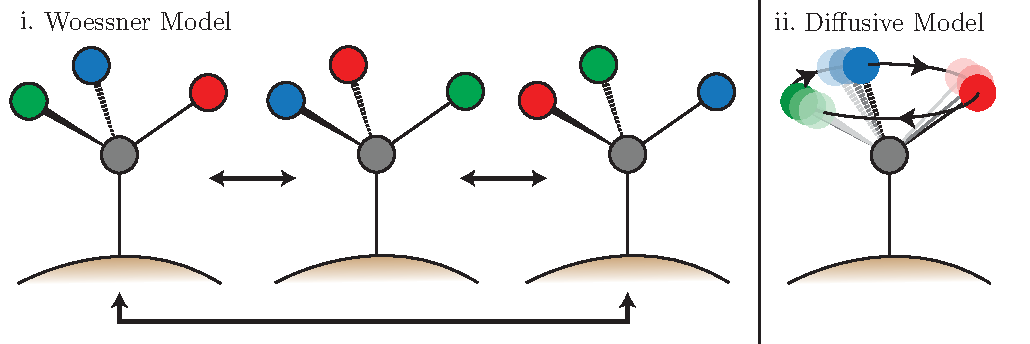
\includegraphics[scale=0.8]{./Figures/SimonsFigs/WoessnerDiffusion.pdf}
\caption{Illustrations of the two types of methyl motion considered in this thesis. i. In the Woessner Model, the three I-spins rapidly exchange between three fixed sites. ii. In the Diffusive Model, the three I-spins are able to rotate freely about a ring, whilst maintaining a their relative orientations to each other.}
\label{WoessnerDiffusive}
\end{figure}
The correlation function adopts the following form\cite{RN4}:
\begin{equation}
\overline{\mathfrak{D}_{k_1,k_1}^{(2) \text{m}*}(t) \mathfrak{D}_{k_2,k_2}^{(2) \text{m}} (t - \tau)} = \delta_{k_1,k_2} e^{-\frac{k_{\text{DW}}^2 \tau}{\tau_{\text{m}}}}
\end{equation}
The constant $k_{\text{DW}}$ adopts different values depending on the model adopted, which are given in Table \ref{kDW}.
\begin{table}[]
\centering
\begin{tabular}{l|l|l}
$k$     & $k_{\text{DW}}$, Woessner & $k_{\text{DW}}$, Diffusive \\ \hline
$0$     & $0$                       & $0$                        \\
$\pm 1$ & $\pm 1$                   & $\pm 1$                    \\
$\pm 2$ & $\pm 1$                   & $\pm 2$                   
\end{tabular}
\caption{The values adopted by the constant, $k_{\text{DW}}$, which is dependent of the value of $k$, and the methyl rotation model considered.}
\label{kDW}
\end{table}
Accounting for these identities, the expression for $\hat{\hat{\Gamma}}$ collapses to:
\begin{equation}
\begin{split}
\hat{\hat{\Gamma}} = &\frac{6}{5} \sum \limits_{i_1, i_2} A_{\text{aniso}}^{i_1} A_{\text{aniso}}^{i_{2}} \sum \limits_{k = -2}^2 \sum \limits_{n_1, n_2} \mathfrak{D}_{k,0}^{(2)*} (\Omega_{i_1}) \mathfrak{D}_{k,0}^{(2)} (\Omega_{i_2}) \\
&\comm{\hat{T}_{i_1, k, n_1}^{(2) \dagger}}{\comm{\hat{T}_{i_2, k, n_2}^{(2)}}{}}\int \limits_0^{\infty} e^{-\frac{\tau}{\tau_{\text{c}}}} e^{-\frac{k_{\text{DW}}^2 \tau}{\tau_{\text{m}}}} e^{-i \omega_{k, n_2} \tau} d \tau \\
= &\frac{6}{5} \sum \limits_{i_1, i_2} A_{\text{aniso}}^{i_1} A_{\text{aniso}}^{i_{2}} \sum \limits_{k = -2}^2 \mathfrak{D}_{k,0}^{(2)*} (\Omega_{i_1}) \mathfrak{D}_{k,0}^{(2)} (\Omega_{i_2}) \\
&\sum \limits_{n_1, n_2} \comm{\hat{T}_{i_1, k, n_1}^{(2) \dagger}}{\comm{\hat{T}_{i_2, k, n_2}^{(2)}}{}} J\left(\frac{\tau_{\text{c}} \tau_{\text{m}}}{\tau_{\text{m}} + \tau_{\text{c}} k_{\text{DW}}^2}, \omega_{k,n_2}\right)
\end{split}
\end{equation}
where $J\left(\frac{\tau_{\text{c}} \tau_{\text{m}}}{\tau_{\text{m}} + \tau_{\text{c}} k_{\text{DW}}^2}, \omega_{k,n_2}\right)$, the spectral density function for this model, is given by:
\begin{equation}
\label{SpecDenMeth}
J\left(\frac{\tau_{\text{c}} \tau_{\text{m}}}{\tau_{\text{m}} + \tau_{\text{c}} k_{\text{DW}}^2}, \omega_{k,n_2}\right) = \frac{\frac{\tau_{\text{c}} \tau_{\text{m}}}{\tau_{\text{m}} + \tau_{\text{c}} k_{\text{DW}}^2}}{1 + \left(\frac{\tau_{\text{c}} \tau_{\text{m}}}{\tau_{\text{m}} + \tau_{\text{c}} k_{\text{DW}}^2}\right)^2 \omega_{k,n_2}^2}
\end{equation}
With the theory established, the attention now moves to comparing the relaxation models outlined in this chapter, along with models already presented in the literature. The next chapter outlines some theoretical relaxation rate calculations on I$_3$S spin systems that have been conducted in an attempt to achieve this. After this, some calculations comparing relaxation in $^{13}$CH$_3$ and $^{13}$CF$_3$ moieties are used to predict the viability of a trifluoromethyl moiety as an effective TROSY probe.